\documentclass[11pt,a4paper]{article}

% ---- Packages ----------------------------------------------------------
\usepackage[utf8]{inputenc}
\usepackage[T1]{fontenc}
\usepackage{lmodern}
\usepackage[margin=0.85in]{geometry}
\usepackage{microtype}
\usepackage{amsmath}
\usepackage{amssymb}
\usepackage{titlesec}
\usepackage{enumitem}
\usepackage{booktabs}
\usepackage{array}
\usepackage{tabularx}
\usepackage{xcolor}
\usepackage{graphicx}
\usepackage{fancyhdr}
\usepackage{tikz}
\usetikzlibrary{positioning, arrows.meta, shapes.geometric, fit, calc, backgrounds, decorations.pathreplacing}
\usepackage[hidelinks,colorlinks=true,linkcolor=black,citecolor=violet,urlcolor=violet]{hyperref}
\usepackage{parskip}
\usepackage{float}
\usepackage{tcolorbox}
\tcbuselibrary{skins, breakable}

% ---- Colours -----------------------------------------------------------
\definecolor{primary}{HTML}{4338CA}
\definecolor{primarylight}{HTML}{E0E7FF}
\definecolor{secondary}{HTML}{0E7490}
\definecolor{secondarylight}{HTML}{CFFAFE}
\definecolor{accent}{HTML}{C2410C}
\definecolor{accentlight}{HTML}{FFEDD5}
\definecolor{ink}{HTML}{1E1B4B}
\definecolor{mute}{HTML}{64748B}
\definecolor{mutelight}{HTML}{F1F5F9}
\definecolor{precfp}{HTML}{0F766E}
\definecolor{precfplight}{HTML}{CCFBF1}
\definecolor{precint}{HTML}{7C3AED}
\definecolor{precintlight}{HTML}{EDE9FE}
\definecolor{ok}{HTML}{15803D}
\definecolor{warn}{HTML}{B91C1C}

% ---- TikZ styles -------------------------------------------------------
\tikzset{
  block/.style    = {rectangle, rounded corners=3pt, draw=primary, thick,
                     fill=primarylight, minimum width=2.6cm, minimum height=0.85cm,
                     align=center, font=\small},
  data/.style     = {rectangle, rounded corners=3pt, draw=mute, thick,
                     fill=mutelight, minimum width=2.4cm, minimum height=0.8cm,
                     align=center, font=\small},
  result/.style   = {rectangle, rounded corners=3pt, draw=accent, thick,
                     fill=accentlight, minimum width=2.4cm, minimum height=0.8cm,
                     align=center, font=\small},
  decision/.style = {diamond, draw=accent, thick, fill=accentlight, aspect=1.6,
                     inner sep=1pt, align=center, font=\small},
  ar/.style       = {-{Latex[length=2mm,width=1.6mm]}, thick, draw=ink!75},
  dar/.style      = {-{Latex[length=2mm,width=1.6mm]}, thick, draw=ink!75, dashed},
}

% ---- Header / Footer ---------------------------------------------------
\pagestyle{fancy}
\fancyhf{}
\fancyhead[L]{\small\color{primary}\textbf{Feature Significance \& Cluster Geometry}}
\fancyhead[R]{\small\color{mute}Madhav Dogra}
\fancyfoot[C]{\small\color{mute}\thepage}
\renewcommand{\headrulewidth}{0pt}

% ---- Section format ----------------------------------------------------
\titleformat{\section}
  {\normalfont\LARGE\bfseries\color{primary}}
  {\textcolor{accent}{\thesection}\hspace{0.4em}}{0pt}{}
\titlespacing*{\section}{0pt}{14pt}{6pt}

\titleformat{\subsection}
  {\normalfont\large\bfseries\color{ink}}
  {\textcolor{secondary}{\thesubsection}\hspace{0.3em}}{0pt}{}
\titlespacing*{\subsection}{0pt}{8pt}{2pt}

\setlength{\parskip}{4pt}

\tcbset{
  idea/.style={colback=secondarylight, colframe=secondary!60, boxrule=0.5pt,
               arc=2pt, left=8pt, right=8pt, top=5pt, bottom=5pt,
               fonttitle=\bfseries\small, coltitle=white, colbacktitle=secondary,
               title={\strut KEY POINT}},
  warnbox/.style={colback=accentlight, colframe=accent!60, boxrule=0.5pt,
                  arc=2pt, left=8pt, right=8pt, top=5pt, bottom=5pt,
                  fonttitle=\bfseries\small, coltitle=white, colbacktitle=accent,
                  title={\strut WATCH OUT}},
}

% =======================================================================
\begin{document}

\begin{center}
{\color{primary}\rule{\linewidth}{1pt}}\\[6pt]
{\Huge\bfseries\color{ink} Feature Significance \& Cluster Geometry} \\[6pt]
{\Large\color{secondary} Visualisation, feature transforms, and the anomaly sphere for the Mamba IoT detector} \\[4pt]
{\color{mute}\rule{0.6\linewidth}{0.3pt}}\\[4pt]
{\normalsize\color{mute} Madhav Dogra}
\end{center}

\vspace{4pt}

% =======================================================================
\section{Finding the features that matter}

t-SNE and its faster cousin UMAP are \textbf{visualisation} tools, not feature rankers. They answer ``do the classes separate?'', not ``which input dimensions made them separate?'' --- and reading a feature ranking off a t-SNE plot is the mistake to avoid.

\begin{tcolorbox}[idea]
t-SNE does not rank input dimensions. Its two output axes are nonlinear blends of \emph{all} the inputs --- there are no per-feature loadings to read off, unlike PCA. So the workflow is: \textbf{rank} features with mutual information and SHAP (both already in the pipeline), then use \textbf{t-SNE / UMAP to \emph{confirm}} that the kept features --- and the learned embeddings --- actually separate the classes.
\end{tcolorbox}

\subsection{What a t-SNE plot can and cannot tell you}
It \emph{can} show whether benign traffic and each attack category fall into distinct clusters --- a fast, honest check that the representation carries class signal. It \emph{cannot} tell you ``feature 7 matters, feature 12 does not,'' because the embedding mixes every input together. Two further cautions: cluster \emph{sizes} and the \emph{distances between} clusters in a t-SNE plot are not meaningful (only local neighbourhoods are preserved), and the picture changes with the perplexity setting. Treat it as a qualitative diagnostic, never as a measurement.

\subsection{Where the ranking comes from}
Three supervised tools answer ``which dimensions matter,'' and all three are already compatible with this project:
\begin{itemize}[leftmargin=*, itemsep=2pt]
  \item \textbf{Mutual information} --- already the feature-selection step in the proposal. Univariate, model-free, ranks each feature by how much it tells you about the label.
  \item \textbf{SHAP} --- already in the design for explainability. It doubles as a global feature-importance ranking by averaging $|$attribution$|$ across flows.
  \item \textbf{Permutation importance} --- shuffle one feature, measure the accuracy drop; a cheap model-agnostic cross-check.
\end{itemize}

\subsection{The right division of labour for this model}
Hand-selecting input dimensions applies to the \textbf{classical baselines} (XGBoost / Isolation Forest on the $\approx$80 aggregated statistics). The \textbf{Mamba} arm does not take a hand-picked feature vector --- it consumes the ordered per-packet sequence and learns its own representation $\mathbf{z}$. For that arm, the high-value use of t-SNE/UMAP is to visualise $\mathbf{z}$ coloured by class: it tells you whether the encoder learned a separable space, which is exactly the precondition the deep-SVDD anomaly head depends on (\S3).

% ---- Figure 1: rank then visualise ------------------------------------
\begin{figure}[H]
\centering
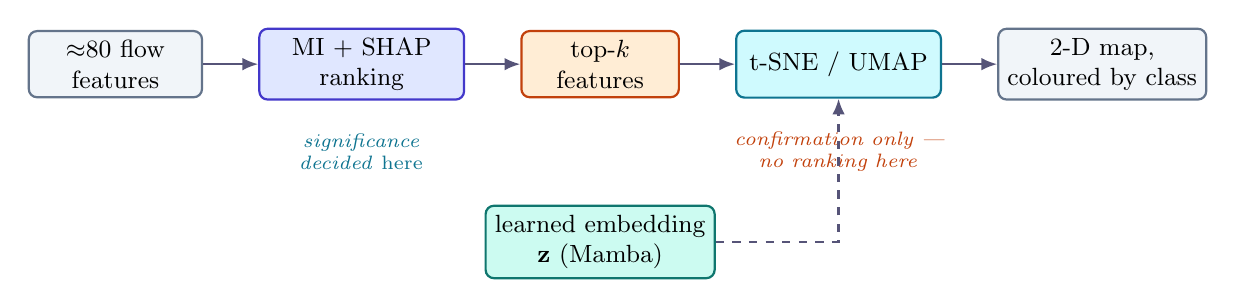
\begin{tikzpicture}[node distance=0.55cm and 0.7cm]

  \node[data, minimum width=2.2cm] (feats) {$\approx$80 flow \\ features};
  \node[block, right=of feats, fill=primarylight, draw=primary] (rank) {MI $+$ SHAP \\ ranking};
  \node[result, right=of rank, minimum width=2.0cm] (topk) {top-$k$ \\ features};
  \node[block, right=of topk, fill=secondarylight, draw=secondary] (tsne) {t-SNE / UMAP};
  \node[data, right=of tsne, minimum width=2.4cm] (map) {2-D map, \\ coloured by class};

  \draw[ar] (feats) -- (rank);
  \draw[ar] (rank) -- (topk);
  \draw[ar] (topk) -- (tsne);
  \draw[ar] (tsne) -- (map);

  \node[font=\scriptsize\itshape\color{secondary}, below=0.3cm of rank, align=center, text width=2.6cm]
       {significance decided \emph{here}};
  \node[font=\scriptsize\itshape\color{accent}, below=0.3cm of tsne, align=center, text width=2.6cm]
       {confirmation only --- \\ no ranking here};

  % Mamba branch
  \node[result, below=1.35cm of topk, fill=precfplight, draw=precfp, minimum width=2.6cm] (z)
       {learned embedding \\ $\mathbf{z}$ (Mamba)};
  \draw[dar] (z.east) -| (tsne.south);

\end{tikzpicture}
\caption*{\small\textit{Figure 1 --- Rank, then visualise. Feature significance is produced by mutual information and SHAP (indigo); t-SNE/UMAP (teal) only \emph{confirms} that the kept features separate the classes --- it never produces the ranking. For the Mamba arm there is no hand-picked vector: the same plot is applied to the learned embedding $\mathbf{z}$ (dashed teal branch) to check the encoder built a separable space.}}
\end{figure}

% =======================================================================
\section{Transforms that compact the clusters}

Raw traffic features need a nonlinear transform before any distance-based clustering or scoring. The transform that compacts them is the logarithm, and the direction is not interchangeable.

\begin{tcolorbox}[idea]
IoT traffic features (packet sizes, byte counts, inter-arrival times) are \textbf{heavy-tailed}, spanning many orders of magnitude. Applying $\log(1+x)$ compresses that tail, makes the distribution near-symmetric, and tightens each class cluster. Standardise (zero-mean, unit-variance) \emph{after} the log, then feed the model.
\end{tcolorbox}

\subsection{Why traffic features are heavy-tailed}
A handful of flows carry megabytes; most carry a few hundred bytes. A few connections idle for seconds between packets; most are sub-millisecond. Raw, these features have a long right tail that dominates any distance computation --- a single bulk transfer sits ``infinitely'' far from everything else, and clustering or one-class scoring is swamped by that one axis. The log pulls the tail back in so the structure of the bulk of the data becomes visible.

\subsection{Direction matters --- log compacts, $\exp$ does the opposite}
\begin{tcolorbox}[warnbox]
$\log$ and $\exp$ move data in \emph{opposite} directions. For positive, right-skewed traffic features, $\log$ compresses large values toward the bulk (good); $e^{x}$ \emph{expands} them and stretches the tail further (worse). Use $\exp$ only on data that is already in log-space or left-skewed --- which these features are not. The compacting transform here is the logarithm, not the exponential.
\end{tcolorbox}

% ---- Figure 2: distribution compaction --------------------------------
\begin{figure}[H]
\centering
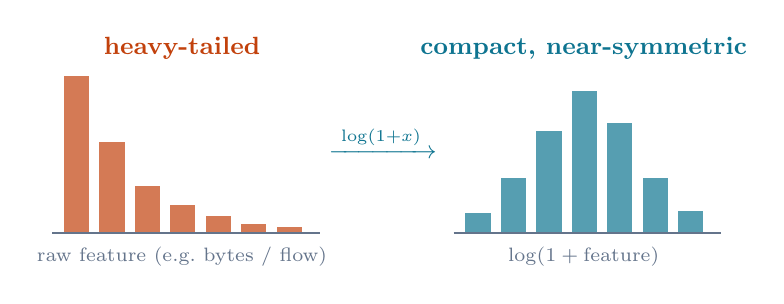
\begin{tikzpicture}

  % ----- raw heavy-tailed -----
  \begin{scope}
    \foreach \x/\h in {0/2.0, 0.45/1.15, 0.9/0.6, 1.35/0.35, 1.8/0.22, 2.25/0.12, 2.7/0.07}
       {\fill[accent!70] (\x,0) rectangle ++(0.32,\h);}
    \draw[mute, thick] (-0.15,0) -- (3.25,0);
    \node[font=\scriptsize\color{mute}] at (1.5,-0.3) {raw feature (e.g.\ bytes / flow)};
    \node[font=\bfseries\small\color{accent}] at (1.5, 2.35) {heavy-tailed};
  \end{scope}

  % arrow
  \node[font=\small\color{secondary}] at (4.05, 1.15) {$\xrightarrow{\;\log(1+x)\;}$};

  % ----- after log1p -----
  \begin{scope}[shift={(5.1,0)}]
    \foreach \x/\h in {0/0.25, 0.45/0.7, 0.9/1.3, 1.35/1.8, 1.8/1.4, 2.25/0.7, 2.7/0.28}
       {\fill[secondary!70] (\x,0) rectangle ++(0.32,\h);}
    \draw[mute, thick] (-0.15,0) -- (3.25,0);
    \node[font=\scriptsize\color{mute}] at (1.5,-0.3) {$\log(1+\text{feature})$};
    \node[font=\bfseries\small\color{secondary}] at (1.5, 2.35) {compact, near-symmetric};
  \end{scope}

\end{tikzpicture}
\caption*{\small\textit{Figure 2 --- The log transform on a heavy-tailed traffic feature. The long right tail (amber) is pulled into a compact, roughly symmetric distribution (teal), so distances and one-class scores reflect the bulk of the data rather than a few outliers. The exponential would push the tail the other way.}}
\end{figure}

\subsection{Yeo--Johnson --- the principled generalisation}
Rather than commit to a fixed $\log$, the \textbf{Yeo--Johnson} power transform learns the best exponent per feature from the data and handles zeros and negatives automatically (unlike a bare $\log$, which needs the $+1$ offset and positive inputs). It subsumes ``log-ish'' and ``mild power'' transforms in one fitted step, and is one \texttt{scikit-learn} call. Recommended default for the aggregated-statistics features; $\log(1+x)$ is the simple, transparent fallback to quote in the report.

% =======================================================================
\section{The anomaly sphere --- compactness done right}

``Everything inside the unit hypersphere is in-class, everything outside is not'' is the principle the anomaly head already implements --- this is Deep SVDD. The subtlety is the mechanism that produces the sphere.

\begin{tcolorbox}[idea]
``Pull normal data into a tight ball; inside $=$ normal, outside $=$ anomaly'' \emph{is} Deep SVDD --- already the anomaly head in the proposal. What builds that ball is a \textbf{learned projection trained on the SVDD objective}, not a scalar $\log$/$\exp$ applied to one normalised input. A single scalar nonlinearity cannot carve a meaningful boundary in a high-dimensional space; the learned transform can.
\end{tcolorbox}

\subsection{What Deep SVDD actually optimises}
Deep SVDD (Ruff et al., 2018) learns a mapping $g_\phi$ that sends benign embeddings as close as possible to a fixed centre $c$ --- it minimises the mean squared distance $\lVert g_\phi(\mathbf{z}) - c\rVert^2$ over benign data, i.e.\ the \emph{volume} of the enclosing sphere. At test time the anomaly score is the distance to $c$; a flow beyond radius $R$ (calibrated at the 99th benign percentile, the 1\% FPR target) is flagged. The compactness is the \emph{training objective itself}, learned jointly with the $\mathbb{R}^{128}\!\to\!\mathbb{R}^{32}$ projection the proposal already specifies to beat distance concentration.

\subsection{The literal unit-sphere variant}
If the goal is points living \emph{on} a unit sphere, that is \textbf{L2 normalisation}: dividing each embedding by its norm puts every point on the unit sphere's \emph{surface}. ``Normal vs anomalous'' then becomes an \textbf{angular} decision --- a spherical cap (cosine similarity to a benign prototype above a threshold) is in-class; the rest of the surface is out. This is the contrastive-learning flavour of the same idea and a clean variant to A/B against radial Deep SVDD. Note the subtlety: normalising alone puts \emph{everything} on the sphere --- you still need a learned threshold (the cap) to separate in- from out-of-class.

\subsection{Why a scalar transform is not enough}
Normalising one feature and pushing it through $\log$ or $\exp$ rescales a single axis; it cannot bend the decision surface that separates ``normal'' from ``everything else'' in a 32-dimensional space. The boundary has to be \emph{learned}. The chain is: log-transform the inputs (\S2) to make the raw space well-behaved, then let the learned projection $+$ SVDD form the sphere.

% ---- Figure 3: the anomaly sphere -------------------------------------
\begin{figure}[H]
\centering
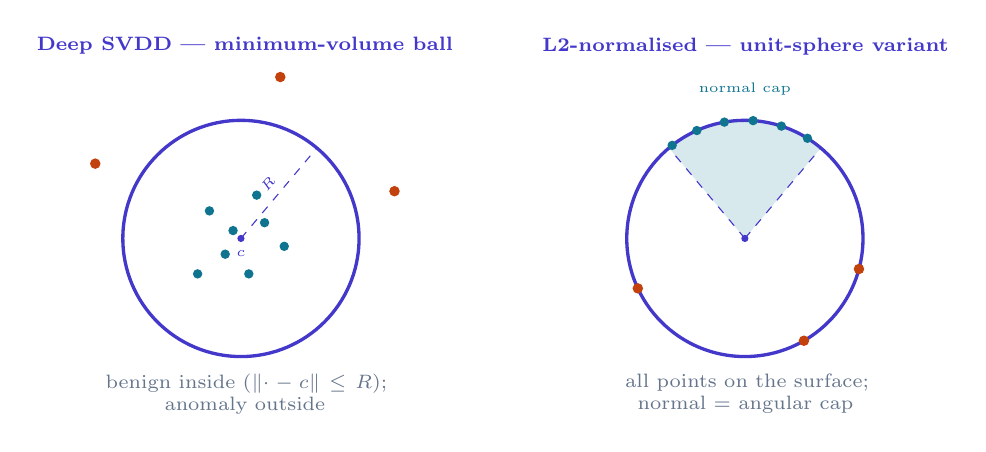
\begin{tikzpicture}

  % ----- Panel A: Deep SVDD ball -----
  \begin{scope}[local bounding box=PA]
    \draw[primary, very thick] (0,0) circle (1.5cm);
    \draw[primary, dashed] (0,0) -- (50:1.5)
         node[midway, above, sloped, font=\tiny\color{primary}] {$R$};
    \fill[primary] (0,0) circle (1.3pt) node[below=1pt, font=\tiny\color{primary}] {$c$};
    \foreach \p in {(0.3,0.2),(-0.4,0.35),(0.1,-0.45),(-0.2,-0.2),(0.55,-0.1),(-0.55,-0.45),(0.2,0.55),(-0.1,0.1)}
       {\fill[secondary] \p circle (1.7pt);}
    \foreach \p in {(1.95,0.6),(-1.85,0.95),(0.5,2.05)}
       {\fill[accent] \p circle (1.9pt);}
  \end{scope}
  \node[font=\bfseries\scriptsize\color{primary}, above=0.1cm of PA] {Deep SVDD --- minimum-volume ball};
  \node[font=\scriptsize\color{mute}, below=0.1cm of PA, text width=4cm, align=center]
       {benign inside ($\lVert\cdot - c\rVert \le R$); \\ anomaly outside};

  % ----- Panel B: L2-normalised unit sphere -----
  \begin{scope}[shift={(6.4,0)}, local bounding box=PB]
    \fill[secondary!16] (0,0) -- (50:1.5) arc (50:130:1.5) -- cycle;
    \draw[primary, very thick] (0,0) circle (1.5cm);
    \draw[primary, dashed] (0,0) -- (50:1.5);
    \draw[primary, dashed] (0,0) -- (130:1.5);
    \foreach \a in {58,72,86,100,114,128} {\fill[secondary] (\a:1.5) circle (1.7pt);}
    \foreach \a in {-15,205,300} {\fill[accent] (\a:1.5) circle (1.9pt);}
    \fill[primary] (0,0) circle (1.3pt);
    \node[font=\tiny\color{secondary}, above] at (90:1.7) {normal cap};
  \end{scope}
  \node[font=\bfseries\scriptsize\color{primary}, above=0.1cm of PB] {L2-normalised --- unit-sphere variant};
  \node[font=\scriptsize\color{mute}, below=0.1cm of PB, text width=4cm, align=center]
       {all points on the surface; \\ normal $=$ angular cap};

\end{tikzpicture}
\caption*{\small\textit{Figure 3 --- Two ways to realise ``inside $=$ in-class.'' Left: Deep SVDD learns a projection that packs benign embeddings (teal) into a minimum-volume ball of radius $R$ around centre $c$; anomalies (amber) fall outside. Right: L2 normalisation places every point on the unit sphere's surface, and ``normal'' becomes a learned angular cap. Both boundaries are \emph{learned} from benign data --- a scalar $\log$/$\exp$ cannot produce either.}}
\end{figure}

% =======================================================================
\section{Summary}

\begin{enumerate}[leftmargin=*, itemsep=3pt]
  \item \textbf{Transform with $\log(1+x)$ or Yeo--Johnson} on the heavy-tailed features before standardising --- not $\exp$, which pushes the wrong way.
  \item \textbf{Rank features with mutual information and SHAP.} Use t-SNE / UMAP only to confirm separability --- of the selected features, and of the learned embedding $\mathbf{z}$.
  \item \textbf{The compact-hypersphere boundary is the Deep-SVDD head} (projection $+$ SVDD objective); optionally A/B against the L2-normalised angular variant.
\end{enumerate}

Two experiments settle this once data lands: (a) t-SNE/UMAP of the features \emph{with} vs.\ \emph{without} the log transform, coloured by class, to \emph{see} the clusters tighten; (b) the same plot on the learned embeddings, to validate the space the anomaly sphere is fitted in.

% =======================================================================
\section*{Pointers}
\footnotesize
\begin{itemize}[leftmargin=*, itemsep=1pt]
  \item \textbf{t-SNE}, van der Maaten \& Hinton, JMLR 2008 --- visualisation, not feature selection.
  \item \textbf{UMAP}, McInnes et al.\ 2018 --- \href{https://arxiv.org/abs/1802.03426}{arxiv.org/abs/1802.03426} --- faster, preserves more global structure.
  \item \textbf{Deep SVDD}, Ruff et al.\ ICML 2018 --- minimum-volume hypersphere one-class objective.
  \item \textbf{Yeo--Johnson} power transform, 2000 --- handles zeros/negatives; \texttt{sklearn.preprocessing.PowerTransformer}.
  \item \textbf{SHAP}, Lundberg \& Lee, NeurIPS 2017 --- attributions that double as feature importance.
\end{itemize}

\end{document}
